% Generated from committed aggregates; insert inside the relevant report section.
\subsection{Final findings}

The final period has 7,783 cell-days, 181 dates and 49 positive next-day targets (0.63\%); these are not independent fires. Both frozen development recall targets failed to transfer \cite{mlFinalEvidence}.

\begin{center}\small\setlength{\tabcolsep}{3pt}
\begin{tabular}{p{0.241\linewidth}p{0.086\linewidth}p{0.138\linewidth}p{0.086\linewidth}p{0.155\linewidth}p{0.155\linewidth}}
\hline
Frozen policy & TP & FP & FN & Recall & Precision \\ \hline
80\% target & 16 & 39 & 33 & 32.7\% & 29.1\% \\
90\% target & 34 & 2,434 & 15 & 69.4\% & 1.4\% \\
Persistence & 16 & 39 & 33 & 32.7\% & 29.1\% \\
\hline\end{tabular}\end{center}

\begin{center}\small\setlength{\tabcolsep}{3pt}
\begin{tabular}{p{0.387\linewidth}p{0.155\linewidth}p{0.163\linewidth}p{0.155\linewidth}}
\hline
Model at diagnostic 0.5 & AP & Recall & Brier \\ \hline
Training prevalence & 0.0063 & 0.0\% & 0.0065 \\
Persistence & 0.0992 & 32.7\% & 0.0093 \\
Logistic 16 & 0.0461 & 81.6\% & 0.1319 \\
Logistic 17 & 0.2113 & 63.3\% & 0.0391 \\
XGBoost 16 & 0.0219 & 57.1\% & 0.1912 \\
XGBoost 17 & 0.1062 & 32.7\% & 0.1511 \\
\hline\end{tabular}\end{center}

\begin{figure}[htbp]\centering
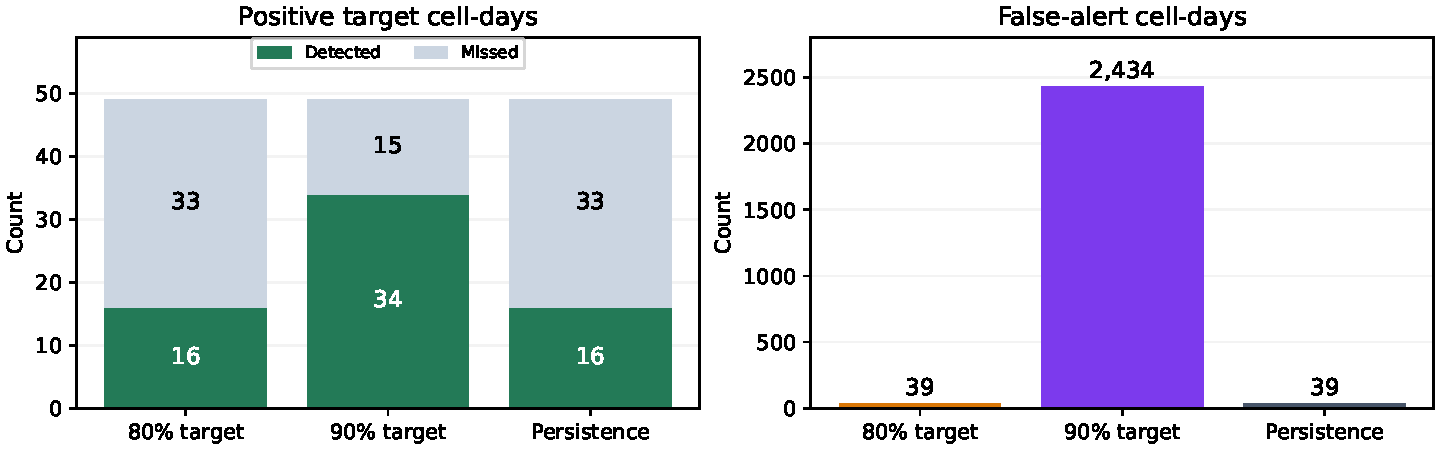
\includegraphics[width=0.94\linewidth]{report/figures/final_policy_tradeoff.pdf}
\caption{Frozen-policy trade-off. Counts are cell-days, not incidents or staffing requirements. The development target is not a promise of final recall.}
\end{figure}

The prespecified logistic 17 comparison ranked better than XGBoost 17; this did not trigger a replacement or retuning. Without current detections, the higher cutoff found 0 of 33 positives; the lower found 18 with 2,395 false alerts. All months were retained, including zero-positive months with undefined AP/recall. A no-alert reference scored 99.37\% accuracy while missing every positive.
